\documentclass[twoside,11pt]{homework}

\usepackage{dsfont}
\usepackage{amsmath}
\usepackage{graphicx}
\usepackage{float}
\usepackage{mathtools}
\DeclarePairedDelimiter{\ceil}{\lceil}{\rceil}

\coursename{COMS 4771 Machine Learning (Spring 2020)} 

\studname{Angela Wang}     
\studmail{aw3062@columbia.edu}
\collab{Jane Pan (jp3740), Stan Liao (sl4239)}
\hwNo{1}      
\date{02/28/2020}  
\begin{document}
\maketitle

\section*{Problem 1} 
\subsection*{(i)}
	\begin{proof}
		Let $y := \text{sign} \left(\sum_{i=1}^{r}x_{k_i}\right)$, $\vec{x} := (x_1,\dots,x_d)$.
		A positive example makes a mistake when $y=1$ and $\hat{y}=0$. We know that
		\begin{align*}
			y=1 &\Longleftrightarrow \sum_{i=1}^{r}x_{k_i} \geq 1 \\
			\hat{y}=0 &\Longleftrightarrow \sum_{k=1}^{d} w_k \cdot x_{k} \leq d \\
			&\Longleftrightarrow \sum_{k: \,x_k=1} w_k  \leq d
		\end{align*}
		And that each update in $\vec{w}$ will result in
		\begin{align*}
			\sum_{k: \,x_k=1} w_k^{(t+1)}  = \sum_{k: \,x_k=1} 2w_k^{(t)},
		\end{align*}
		until the program moves to the next example when $\sum_{k: \,x_k=1} w_k  > d$. 
		In the worst case, $\sum_{k: \,x_k=1} w_k$ should increase as slow as possible.
		We thus only consider examples with $\sum_{i=1}^{r}x_{k_i}=\sum_{k=1}^{d} x_{k}=1$.
		In other words, examples $\vec{x}$ that have only one non-zero field, 
		which is in one of the fields selected by the OR operation.
		There are in total $r$ examples we should consider.\\
		For each example $\vec{x}$, $\exists i $ such that $x_{k_i} = 1$. 
		The condition for making a mistake is therefore written as
		\begin{align*}
			w_{k_i}  &\leq d
		\end{align*}
		Let $T$ be the minimum number of steps required to pass this type of example. 
		Since $w_{k_i} ^{(0)} = 1$ and $w_{k_i} ^{(t+1)} = 2w_{k_i} ^{(t)} $, we have
		\begin{align*}
			w_{k_i}^{(T)} =  2^T w_{k_i}^{(0)} =  2^T \leq d \\
			T\leq \ceil{\log{d}} < \log{d}+1
		\end{align*}
		Since there are at most $r$ examples with $x_{k_i} = 1$ and $x_k = 0$ $\forall k \neq k_i$. 
		The total number of steps required should be at most $rT \leq r(\log{d} + 1)$.
		Upon seeing other positive examples, there will be no more mistakes, since $\vec{w}\cdot\vec{x}$ will always be greater than $d$.
	\end{proof}

\subsection*{(ii)}
	\begin{proof}
		A negative example makes a mistake when $y=0$ and $\hat{y}=1$. We know that
		\begin{align*}
			y=0 &\Longleftrightarrow \sum_{i=1}^{r}x_{k_i} = 0 \\
			\hat{y}=1 &\Longleftrightarrow \sum_{k=1}^{d} w_k \cdot x_{k} > d \\
			&\Longleftrightarrow \sum_{k: \,x_k=1} w_k  > d
		\end{align*}
		And that each update in $\vec{w}$ will result in
		\begin{align*}
			\sum_{k: \,x_k=1} w_k^{(t+1)}  &= \sum_{k: \,x_k=1} \frac{1}{2}w_k^{(t)}
			= \frac{1}{2} \sum_{k: \,x_k=1} w_k^{(t)}  \\
			\sum_{k: \,x_k=0} w_k^{(t+1)}& = \sum_{k: \,x_k=0} w_k^{(t+1)}
		\end{align*}
		Therefore,
		\begin{align*}
			\sum_{k=1}^d w_k^{(t+1)}-\sum_{k=1}^d w_k^{(t)}  
			= \frac{1}{2} \sum_{k: \,x_k=1} w_k^{(t)}
			> \frac{d}{2}
		\end{align*}
	\end{proof}

\subsection*{(iii)}
	\begin{proof}
		Since $w_k = 1$ $\forall k = 1,\dots, d$, and each update in $\vec{w}$ multiplies its fields by a positive constant,
		we know that
		\begin{align*}
			\sum_{k=1}^d w_k ^{(t)} > 0
		\end{align*}
		We observe that each mistake made on a positive example increases the total weight by at most $d$, since
		\begin{align*}
			\sum_{k: \,x_k=1} w_k^{(t+1)}  &= \sum_{k: \,x_k=1} 2w_k^{(t)} \\
			\sum_{k: \,x_k=0} w_k^{(t+1)}  &= \sum_{k: \,x_k=0} w_k^{(t)} \\
			\sum_{k=1}^d w_k^{(t+1)}-\sum_{k=1}^d w_k^{(t)} &=   \sum_{k: \,x_k=1} w_k^{(t)} \leq d
		\end{align*}
		The accumulated change after $t$ iterations in the total weight is 
		\begin{align*}
			\sum_{k=1}^d w_k ^{(t)} -\sum_{k=1}^d w_k ^{(0)} \leq d M_+ -\frac{d}{2} M_-
		\end{align*}
		And we have 1
		\begin{align*}
			0<\sum_{k=1}^d w_k ^{(t)} &\leq  \sum_{k=1}^d w_k ^{(0)}  +d M_+ -\frac{d}{2} M_- \\
			0&<d+ d M_+ -\frac{d}{2} M_-\\
			0&<1+  M_+ -\frac{1}{2} M_-\\
			M_- &<2+  2M_+
		\end{align*}
		Thus, we can write
		\begin{align*}
			M_+ + M_-  < 2+ 3M_+< 2+3r(\log{d}+1)
		\end{align*}
	\end{proof}


\section*{Problem 2}
\subsection*{(i)}
	Suppose we have a perfect classifier such that $\hat{Y}=y$ whenever $Y=y$, 
	and that the distribution of $(X,A,Y)$ is symmetrical across the sensitive attribute $A$. 
	For example, let $(f(X),A,Y)\in \{(1,1,1),(1,0,1),(0,1,0),(0,0,0)\}$ with uniform distribution.
	Thus we have
	\begin{align*}
		\mathbb{P}_0[\hat{Y}=\hat{y}] &= \frac{1}{2} = \mathbb{P}_1 [\hat{Y}=\hat{y}] \tag{DP}  \\
		\mathbb{P}_0[\hat{Y}=1|Y=1] &= 1 = \mathbb{P}_1 [\hat{Y}=1|Y=1] \tag{True Positive EO} \\
		\mathbb{P}_0[\hat{Y}=0|Y=0] &= 1 = \mathbb{P}_1 [\hat{Y}=0|Y=0] \tag{True Negative EO} \\
		\mathbb{P}_0[Y=1 | \hat{Y}=1] &=1 = \mathbb{P}_1[Y=1 | \hat{Y}=1] \tag{Positive PP} \\
		\mathbb{P}_0[Y=0 | \hat{Y}=0] &=1 = \mathbb{P}_1[Y=0 | \hat{Y}=0] \tag{Negative PP}
	\end{align*}
\subsection*{(ii)}
	\begin{proof}
		Suppose both DP and PP are satisfied.
		Then we have 
		\begin{align*}
			\mathbb{P}_0[\hat{Y}=\hat{y}] &= \mathbb{P}_1 [\hat{Y}=\hat{y}] \tag{DP} \\
			\mathbb{P}_0[Y=1 | \hat{Y}=1] &= \mathbb{P}_1[Y=1 | \hat{Y}=1] \tag{Positive PP} \\
		\end{align*}
		Since the random variable $(\hat{Y},A,Y)$ satisfy separation ($\hat{Y}\perp A|Y$), we have
		\begin{align*}
			\mathbb{P}_0[\hat{Y}=1|Y=1] = \mathbb{P}_1[\hat{Y}=1|Y=1] 
		\end{align*}
		By Positive Predicative Parity, we can write
		\begin{align*}
			\mathbb{P}_0[Y=1 | \hat{Y}=1] &= \mathbb{P}_1[Y=1 | \hat{Y}=1] \\
			\frac{\mathbb{P}_0[\hat{Y}=1|Y=1] \mathbb{P}_0[Y=1] }{\mathbb{P}_0[\hat{Y}=1] } 
			&= \frac{\mathbb{P}_1[\hat{Y}=1|Y=1] \mathbb{P}_1[Y=1] }{ \mathbb{P}_1[\hat{Y}=1] } \tag{Bayes Rule} \\
			\mathbb{P}_0[\hat{Y}=1|Y=1] \mathbb{P}_0[Y=1] &= \mathbb{P}_1[\hat{Y}=1|Y=1] \mathbb{P}_1[Y=1] \tag{DP}\\
			\mathbb{P}_0[Y=1] &= \mathbb{P}_1[Y=1] \tag{Separation Condition}
		\end{align*}
		However $A\perp Y$ contradicts the dependence condition.
	\end{proof}
\subsection*{(iii)}
	\begin{proof}
		By Positive Equalized Odds, 
		\begin{align*}
			\mathbb{P}_0[ \hat{Y}=1|Y=1] &= \mathbb{P}_1[\hat{Y}=1|Y=1] \\
			\frac{\mathbb{P}_0[Y=1|\hat{Y}=1] \mathbb{P}_0[\hat{Y}=1] }{\mathbb{P}_0[{Y}=1] } 
			&= \frac{\mathbb{P}_1[Y=1|\hat{Y}=1] \mathbb{P}_1[\hat{Y}=1] }{ \mathbb{P}_1[{Y}=1] } \tag{Bayes Rule} \\
			\frac{\mathbb{P}_0[Y=1|\hat{Y}=1]}{\mathbb{P}_0[{Y}=1] } 
			&= \frac{\mathbb{P}_1[Y=1|\hat{Y}=1]}{ \mathbb{P}_1[{Y}=1] } \tag{DP}\\
			\mathbb{P}_0[Y=1] &= \mathbb{P}_1[Y=1] \tag{$\hat{Y}$ dependent on $Y$}
		\end{align*}
		However $A\perp Y$ contradicts the dependence condition.
	\end{proof}
\subsection*{(iv)}
	\begin{proof}
		Let $\text{PPV}_a := \mathbb{P}_a[Y=1 | \hat{Y}=1]$. We have
		\begin{align*}
			\text{PPV}_a & = \mathbb{P}_a[Y=1 | \hat{Y}=1] \\
			&= \frac{\mathbb{P}_a[\hat{Y}=1|Y=1] \mathbb{P}_a[Y=1] }
			{\mathbb{P}_a[\hat{Y}=1] } \tag{Bayes Rule}\\
			&= \frac{\mathbb{P}_a[\hat{Y}=1|Y=1] \mathbb{P}_a[Y=1] }
			{\mathbb{P}_a[\hat{Y}=1|Y=1] \mathbb{P}_a[Y=1]+
			\mathbb{P}_a[\hat{Y}=1|Y=0] \mathbb{P}_a[Y=0] }\\
			&= \frac{ (1-\mathbb{P}_a[\hat{Y}=0|Y=1]) \mathbb{P}_a[Y=1] }
			{ (1-\mathbb{P}_a[\hat{Y}=0|Y=1])  \mathbb{P}_a[Y=1]+
			\mathbb{P}_a[\hat{Y}=1|Y=0] (1-\mathbb{P}_a[Y=1]) }\\
			&= \frac{(1-\text{FNR}_a) p_a}{(1-\text{FNR}_a)  p_a+\text{FPR}_a(1-p_a)}
		\end{align*}
		By Equalized Odds, we have $\text{FNR}_0=\text{FNR}_1$, and $\text{FPR}_0=\text{FPR}_1$.
		By Positive Predictive Parity, $\text{PPV}_0=\text{PPV}_1$ which implies either $\text{FNR}_a=1$ 
		or $\text{FPR}_a=0$. However considering Negative Predictive Parity,
		\begin{align*}
			\text{NPV}_a &=  \mathbb{P}_a[Y=1 | \hat{Y}=0] \\
			&= \frac{\mathbb{P}_a[\hat{Y}=0|Y=1] \mathbb{P}_a[Y=1] }
			{\mathbb{P}_a[\hat{Y}=0] } \tag{Bayes Rule}\\
			&= \frac{\mathbb{P}_a[\hat{Y}=0|Y=1] \mathbb{P}_a[Y=1] }
			{\mathbb{P}_a[\hat{Y}=0|Y=1] \mathbb{P}_a[Y=1]+
			\mathbb{P}_a[\hat{Y}=0|Y=0] \mathbb{P}_a[Y=0] }\\
			&= \frac{\text{FNR}_a p_a}{\text{FNR}_a p_a+(1-\text{FPR}_a)(1-p_a)}
		\end{align*}
		in either case, $\text{NPV}_0\neq \text{NPV}_1$. Hence predictive value parity fails.
	\end{proof}

\section*{Problem 3} 
\subsection*{(i)}
	\begin{proof}
		$\phi_\sigma$ forms an uncountably infinite feature space corresponding in cardinality to $\mathbb{R}$. 
		By the density of rationals, $\forall x_i$ for $i \in [1,n] \exists r \in \mathbb{Q}$  
		s.t. $r$ is not in between $x_i$ and any other members of x. \\
		$\therefore$ we can construct a neighborhood $N$ of radius $\sigma > 0$ about $x_i$ 
		s.t. $\nexists x_j \in N$ where $j \in [1, n]$ and $j \neq i$. \\
		By the conditions of the problem, this means that $\phi_\sigma (x) = 0 \forall x_i$ of our choice. \\
		$\therefore$ we can select a $\sigma$ s.t. any binary labeling of the n points will have one label corresponding to zero values in $\phi_\sigma(x)$ and one label corresponding to nonzero values. We can draw a hyperplane dividing zero from nonzero values in the relevant dimensions (i.e. those corresponding to the $x_i$ of one of our binary labels). This hyperplane can have arbitrary values in the other dimensions. This hyperplane will separate the n points by binary label, thus construing a linear separation. 
	\end{proof}

\subsection*{(ii)}
	\begin{proof}
		By $x \mapsto 1[|\alpha-x| < \sigma]:\\
		\forall \alpha$ s.t. $|\alpha - x| > \sigma $ or $|\alpha - x'| > \sigma$, $\phi_\sigma(x) \phi_\sigma(x') = 0$\\
		Let $A$ be the minimum value of $\alpha$ where $|\alpha - x| < \sigma $ or $|\alpha - x'| < \sigma$\\
		Let $B$ be the maximum value of $\alpha$ where $|\alpha - x| < \sigma $ or $|\alpha - x'| < \sigma$\\
		The only nonzero values of the dot product occurs where $\alpha \in [A, B]$.  Thus, we only hve to integrate from A to B, because the rest of the values are zero.\\
		$\phi_\sigma(x) \dot \phi_\sigma(x') = \int_{A}^{B} \phi_\sigma(x) \phi_\sigma(x') d\alpha$
	\end{proof}

\subsection*{(iii)}
	\subsection*{(a)}
	\begin{proof}
		$ || \phi(x) - c_+ || \leq || \phi(x) - c_-||$ \\ 
		$ \iff  \sqrt{\phi \cdot \phi - 2c_+ \cdot \phi + c_+ \cdot c_+} \leq  \sqrt{\phi \cdot \phi - 2c_- \cdot \phi - c_+ \cdot c_-}$\\
		$ \iff  - 2c_+ \cdot \phi + c_+ \cdot c_+ \leq  - 2c_- \cdot \phi + c_- \cdot c_-$ \\
		$\iff - c_+ \cdot \phi + \frac{1}{2} c_+ \cdot c_+ \leq  - c_- \cdot \phi + \frac{1}{2} c_- \cdot c_- $ \\
		$\iff  c_+ \cdot \phi - c_- \cdot \phi + \frac{1}{2} (-c_+ \cdot c_+  + c_- \cdot c_-) \geq 0$ \\
		$\iff  (c_+ - c_-) \cdot \phi + \frac{1}{2} ( ||c_-||^2 - ||c_+ ||^2) \geq 0$ \\
		$\iff  \langle w, \phi(x) \rangle + b \geq 0$ \\
		$\therefore \langle w, \phi(x) \rangle + b$  is positive iff $h(x)  = 1$ and is negative iff $h(x) = -1$.\\
		$h(x)  =$ sign$( \langle w, \phi(x) \rangle + b)$
	\end{proof}

	\subsection*{(b)}
	$h(x) = 1$ iff $K(w, \phi(x)) \geq \frac{1}{2}(K(c_-, c_-), K(c_+, c_+))$\\
	otherwise, $h(x) = -1$


\section*{Problem 4}
\subsection*{a}
\begin{align*}
	g(t) &= f(tx+(1-t)y)\\
	g'(t) &= (x-y) \frac{d}{dt} f(tx+(1-t)y)\\
	g''(t) &= (x-y)^2\frac{d^2}{dt^2} f(tx+(1-t)y)\\
\end{align*}

\subsection*{b}
\begin{proof}
Taylor's theorem states that if a function and its first n derivatives are continuous on $[a, b]$ or $[b, a]$ (with $f^{(n)}$ differentiable on $(a, b)$ or $(b, a)$, then $\exists$ c s.t.:

\begin{align*}
	f(b) = f(a)+f'(a)(b-a)+\frac{f''(a)}{2!}(b-a)^2 +...+\frac{f^{(n)}(a)}{n!}(b-a)^n+\frac{f^{(n+1)}(c)}{(n+1)!}(b-a)^{n+1}
\end{align*}

Letting $b = 0$, $a = t$, $n=1$, and $c \in (0, t)$:

\begin{align*}
	g(0) &= g(t) + g'(t)(0-t)+\frac{g^{(1+1)(c)}}{2}(0-t)^{1+1}\\
	g(0)&= g(t) + g'(t)(0-t)+\frac{g''(c)}{2}(0-t)^{2}\\
	g(0)-(g(t) + g'(t)(-t)) &= \frac{g''(c)}{2}(-t)^{2}\\
	g(0)-(g(t) + g'(t)(-t)) &= \frac{g''(c)}{2}t^{2}\\
\end{align*}

From part (a) we know that $\forall c \in (0, 1)$, $g''(c) \geq 0$; also, $t^2 \geq 0$. Thus:

\begin{align*}
	g(0)-(g(t) + g'(t)(-t)) &\geq 0\\
	g(0)&\geq g(t) + g'(t)(-t)\\
\end{align*}

Similarly, for $b = 1$:

\begin{align*}
	g(1) &= g(t) + g'(t)(1-t)+\frac{g^{(1+1)(c)}}{2}(1-t)^{1+1}\\
	g(1)&= g(t) + g'(t)(1-t)+\frac{g''(c)}{2}(1-t)^{2}\\
	g(1)-(g(t) + g'(t)(-t)) &= \frac{g''(c)}{2}(1-t)^{2}\\
	g(1)-(g(t) + g'(t)(-t)) &= \frac{g''(c)}{2}(1-t)^{2}\\
\end{align*}

From part (a) we know that $\forall c \in (0, 1)$, $g''(c) \geq 0$; also, $(1-t)^2 \geq 0$. Thus:

\begin{align*}
	g(1)-(g(t) + g'(t)(1-t)) &\geq 0\\
	g(1)&\geq g(t) + g'(t)(1-t)\\
\end{align*}	
\end{proof}

\subsection*{c}
\begin{proof}
	We are given that $g = f(tx+(1-t)y)$. Thus, if f is convex (i.e. $f(tx+(1-t)y)\leq tf(x)+(1-t)f(y)$), this implies that g is also convex.
	
	We note that:
	\begin{align*}
		g(0) &= f(y)\\
		g(1) &= f(x)\\
	\end{align*}
	
	Plugging this into the convexity condition for f gives:
	
	\begin{align*}
		f(tx+(1-t)y)&\leq tf(x)+(1-t)f(y)\\
		g(t)&\leq tg(1)+(1-t)g(0)\\
	\end{align*}
	
	Now recall the inequalities given in part (ii):	
	\begin{align*}
	g(0) &\geq g(t) + g'(t)(-t)\\
	g(1) &\geq g(t) + g'(t)(1-t)\\
	\end{align*}
	
We multiply by $1-t$ and $t$, respectively, and then add:

	\begin{align*}
	(1-t)g(0)+tg(1)&\geq (1-t)[g(t) + (1-t)g'(t)(-t)]+t[g(t) + g'(t)(1-t)]\\
	 &\geq g(t) -t(1-t)g'(t)+ t(1-t)g(t)\\
	 &\geq g(t)\\
	\end{align*}
	
Thus, we have shown that:
\begin{align*}
	g(t)&\leq tg(1)+(1-t)g(0)\\
	f(tx+(1-t)y)&\leq tf(x)+(1-t)f(y)\\
\end{align*}
\end{proof}

\section*{Problem 5}
Notes for me, will delete later:

Papers used: https://arxiv.org/pdf/1609.04747.pdf


"Describe each of the techniques in detail. Compare and contrast the relative advantages and
disadvantages of each of the techniques. Are there specific types of datasets where one technique is expected to perform better than the other? if so, why? Provide detailed justifications
for each."
\subsection*{Full Gradient Descent}
Full gradient descent adjusts the parameters of the model after computing the gradient of the cost function using the following formula:

\begin{align*}
	\theta &= \theta - \eta \nabla_\theta J(\theta)
\end{align*}

Here, $\theta$ are the parameters of the model and $\eta$ is the learning rate. The learning rate controls how much the parameters are changed per update according to the gradient Note that the gradients are calculated for the entire dataset for each update.

\begin{enumerate}
	\item Advantages: GD is guaranteed to converge to a minimum (global if the error surface is convex and local otherwise).
	\item Disadvantages: GD is extremely slow since the gradient must be calculated for the entire dataset for a single update. This means GD is unsuited for very large datasets (especially those that cannot be stored in memory). Moreover, since the entire original dataset must be used to perform updates in GD, new data cannot be added on the fly during training. Also, since the learning rate is chosen and fixed for all parameters, it is difficult to to chose a rate that is neither too small (leading to slow convergence) or too fast (leading to fluctuation around minima or failure to converge) for all parameters. This is particularly difficult when there are many parameters; a common learning rate may make the algorithm take steps that are too big in one dimension (if the contour is steep in that direction), yet are too small in other dimensions (where the contour is relatively flat). If the error surface has many local minima, the error function may be "stuck" in a local minima and will fail to converge to the optimum solution. 
	\item Best used for: Smaller datasets for which the model does not need to be updated online. This is because GD will run too slowly with larger datasets and cannot account for online updates. 
\end{enumerate}

\subsection*{Stochastic Gradient Descent}
Stochastic gradient descent (SGD) adjusts the parameters of the model after computing the gradient of the cost function after each point:

\begin{align*}
	\theta = \theta - \eta \nabla_\theta J(\theta; x^{(i)}; y^{(i)})
\end{align*}
Stochastic gradient descent uses one data point to compute the gradient. Mini-batch gradient descent will use a small sample of multiple points to compute the gradient.
\begin{enumerate}
	\item Advantages: Since the gradients are noisier than that of full batch GD, this is better suited to error surfaces with many local minima since the model may "jump" out of ravines. Since you compute gradients for much fewer points, SGD runs a lot faster than GD. Also, smaller data sets means that there is no need for the entire dataset to be stored in RAM.
	\item Disadvantages: Has the same fallbacks of a fixed learning rate as vanilla GD. Moreover, SGD's weakness lies when the surface curves steeply in one dimension but not steeply in another, forming a ravine or valley-like contour. This will cause the algorithm to "jump" from wall to wall of the ravine while making slow progress along it.
	\item Best used for:
\end{enumerate}

\subsection*{Stochastic Gradient Descent with Momentum}
Stochastic Gradient Descent with Momentum (SGDM) seeks to alleviate the issues caused by ravines in standard SGD by introducing a momentum component. 

\begin{align*}
	v_t &= \gamma v_{t-1} + \eta \nabla_\theta J(\theta)\\
	\theta &= \theta - v_t
\end{align*}
Here, $v_t$ is the update vector which we use to adjust $\theta$ after each iteration. Momentum adds a fraction (the momentum term $\gamma$) of the previous update vector to the current update vector. This means that a dimension of the current update vector is increased when if the direction of the dimension in the current gradient is the same of that in previous gradient. Likewise, it is decreased if the directions are opposite. 


\begin{enumerate}
	\item Advantages: Is better suited than SGD to an error surface with ravines.
	\item Disadvantages: Has the same fallbacks of a fixed learning rate as vanilla GD.
	\item Best used for: Datasets whose error manifolds form ravines.
\end{enumerate}

\subsection*{Adaptive Gradient}
Adaptive gradient (AdaGrad), as its name suggests, adapts the learning rate $\eta$ to each parameter. Common parameters are updated with smaller steps, whereas infrequent parameters are updated with bigger steps.

\begin{align*}
	\theta_{t+1} = \theta_{t} - \frac{\eta}{\sqrt[]{G_{t}+\epsilon}} \nabla_{\theta_t} J(\theta_{t})\\
	G_{ii} = \sum^t_{k=1} (\nabla_{\theta_k} J(\theta_{t, i}))^2
\end{align*}

Here, parameter $\theta_i$ is updated with value $\theta_{t+1, i}$ at time $t+1$. $G_{t, ii}$ is a diagonal matrix with each diagonal term being the sum of the squares of all past gradients. $\epsilon$ is a smoothing term to prevent division by zero.
 

%https://web.archive.org/web/20150330033637/http://seed.ucsd.edu/mediawiki/images/6/6a/Adagrad.pdf
\begin{enumerate}
	\item Advantages: Very useful for sparse data; the G matrix ensures that when uncommon parameters are present, the step size is large in those dimensions, meaning that the model will rapidly adjust even if not much of the data displays that parameter.
	\item Disadvantages: Since gradients are squared and summed, the values in $G_t$ are monotonically increasing. Therefore, since we divide $\eta$ by $G_t$ and the values in $G_t$ continue to grow, eventually the learning rate will shrink to very small values. This will mean that the algorithm's update will barely change the parameters and the algorithm will barely learn more.
	\item Best used for: sparse datasets for the reasons explained above.
\end{enumerate}
\subsection*{RMSProp}
RMSProp (root mean square propagation) is a modification to AdaGrad meant to combat its chief disadvantage: its monotonically decreasing learning rate. 

\begin{align*}
	E[g^2]_t &= \gamma E[g^2]_{t-1} + (1-\gamma)g^2_t\\
	\theta_{t+1} &= \theta_t - \frac{\eta}{\sqrt[•]{E[g^2]_t+\epsilon}} g_t
\end{align*}

RMSProp introduces a term similar to that of the momentum term in SGDM. Here, we divide the learning rate by an exponentially decaying average of the squared gradients. This prevents a situation like the G-matrix we saw earlier (i.e. the learning rate becoming increasingly smaller until the algorithm makes negligible adjustments with each iteration).

\begin{enumerate}
	\item Advantages: Moreover, learning rate is no longer monotonically decreasing, so no need to worry about the algorithm eventually failing to learn.
	\item Disadvantages:
	\item Best used for:
\end{enumerate}
\subsection*{AdaDelta}
AdaDelta, like RMSProp, is a modification to AdaGrad meant to combat its chief disadvantage: its monotonically decreasing learning  rate. It is indeed very similar to RMSProp. In fact, the only difference between them is the usage of the root mean square of the parameter updates, rather than a preset $\eta$. We use $g$ as a shorthand for the gradient at time step $t$, and $E[g^2]_t$ as the running decaying average of the past squared gradients.

\begin{align*}
	g_t &= \nabla_{\theta_t} J(\theta_{t, i})\\
	\theta_{t+1} &= \theta_t + \delta \theta_t\\
	E[g^2]_t &= \gamma E[g^2]_{t-1} + (1-\gamma)g^2_t \\
	E[\Delta \theta^2]_t &= \gamma E[\Delta \theta^2]_{t-1} + (1-\gamma)(\Delta \theta)^2_t \\
	RMS[g]_t &= \sqrt[•]{E[g^2]_t+\epsilon}\\
	RMS[\Delta \theta]_t &= \sqrt[•]{E[\Delta \theta^2]_t+\epsilon}\\
	\theta_{t+1} &= \theta_t - \frac{RMS[\Delta \theta]_{t-1}}{RMS[g]_t} g_t\\
\end{align*}

The reason why we take the 
\begin{enumerate}
	\item Advantages: No need to set default learning rate since it is no longer a component of the update rule; solves the monotonically decreasing learning rate problem presented by AdaGrad.
	\item Disadvantages:
	\item Best used for:
\end{enumerate}
\subsection*{Adaptive Moment Estimation}
Adaptive Moment Estimation (ADAM), like AdaGrad, is a method which uses adaptive learning rates rather than a fixed one. Like Adadelta, ADAM maintains a exponentially decaying average of square gradients, but also adds an exponentially decaying average of past (unsquared) gradients. This acts in a similar fashion to momentum.

\begin{align*}
	m_0 &= 0\\
	v_0 &= 0\\
	m_t &= \beta_1 m_{t-1}+(1-\beta_1)g_t\\
	v_t &= \beta_2 v_{t-1}+(1-\beta_2)g^2_t\\
\end{align*} 

Since the vectors are initialized at zero, $m_t$ and $v_t$ will be biased towards zero, so we use bias-corrected estimates instead:

\begin{align*}
	\hat{m_t} &= \frac{m_t}{1-\beta^t_1}\\
	\hat{v_t} &= \frac{v_t}{1-\beta^t_2}\\
	\theta_{t+1} &= \theta_t - \frac{\eta}{\sqrt[•]{\hat{v}_t+\epsilon}}\hat{m}_t
\end{align*}

\begin{enumerate}
	\item Advantages: Because Adam is a combination of SGD and RMSProp with momentum, Adam works well with sparse gradients and on-line settings. Adam tends to be significantly faster and more powerful than other methods.
	\item Disadvantages: Because Adam is adaptive, it generalizes poorly, especially compared to SGD with momentum when tested on a diverse set of deep learning tasks. Due to its poor generalization, it may fail to converge to an optimal solution. One possible cause is that Adam's learning saturates in later stages of training. The updates of Adam, unlike in SGD, do not lie in the span of historical gradients. Additionally, while the magnitudes of Adam parameter updates are invariant to descaling of the gradient, the effect of the updates on the same overall network function still varies with the magnitudes of parameters.
	\item Best used for: areas with tiny gradients (e.g. saddle points, ravines) because the step size of Adam update rule is invariant to the magnitude of the gradient. Adam is also good for sparse gradients (advantage of Adagrad incorporated by Adam), and in on-line settings (advantage of RMSProp).
\end{enumerate}

\begin{proof}[Proof]
Let $\hat{\eta}$ denote the value that maximizes $L^*(\eta | \textbf{x})$. We must show that $L^*(\hat{\eta} | \textbf{x})=L^*[\tau(\hat{\theta} | \textbf{x}]$.
Now, as stated above, the maxima of $L$ and $L^*$ coincide, so we have:
\[ L^*(\hat{\eta} | \textbf{x})=\sup_{\eta}\sup_{\{\theta :\tau (\theta)=\eta\}}L(\theta | \textbf{x})=\sup_{\theta} L(\theta | \textbf{x})=L(\hat{\theta} | \textbf{x}) \]
where the second equality follows because the iterated maximiazation is equal to the unconditional maximization over $\theta$, which is attained at $\hat{\theta}$. Furthermore
\[ L(\hat{\theta} | \textbf{x}) = \sup_{\{\theta :\tau (\theta)=\tau{\hat{\theta}}\}} L(\theta | \textbf{x}) = L^*[\tau(\hat{\theta}) | \textbf{x}]. \]
Hence, the string of equalities shows that $L^*(\hat{\eta} | \textbf{x}) = L^*(\tau(\hat{\theta}) | \textbf{x})$ and that $\tau(\hat{\theta})$ is the MLE of $\tau(\theta)$.
\end{proof}



\section*{Problem 6}
\subsection*{(ii)}
	The Perceptron Algorithm performs differently under different splits of the dataset. From the plots, we choose
	the ration of training data to be 0.80, 0.75, and 0.85, for V0, V1, V2 respectively.
	\begin{figure}[H]
		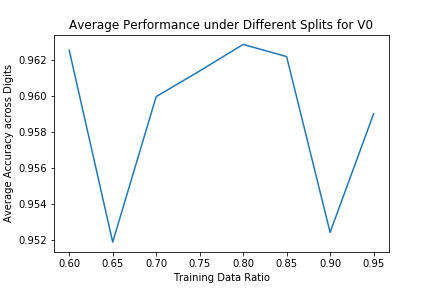
\includegraphics[scale=0.6]{q6/img/splits_v0_smoothed.png}\\
		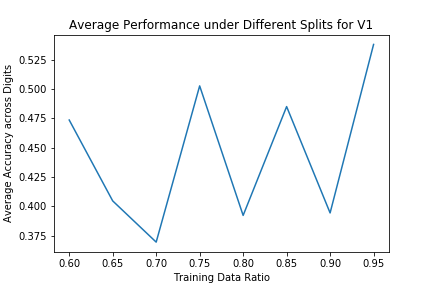
\includegraphics[scale=0.6]{q6/img/splits_v1_smoothed.png}\\
		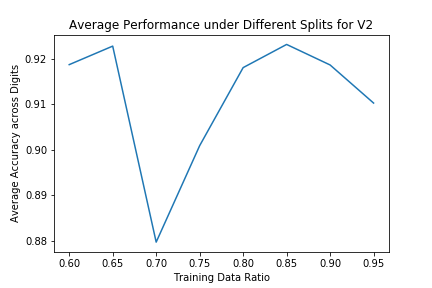
\includegraphics[scale=0.6]{q6/img/splits_v2.png}
	\end{figure}
	
	\begin{figure}[H]
		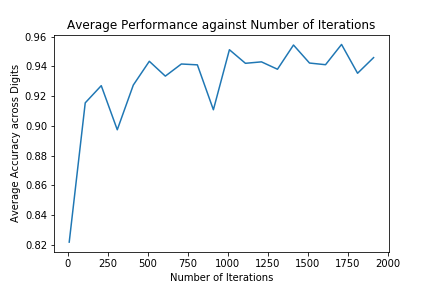
\includegraphics[]{q6/img/iterations_v0.png}
		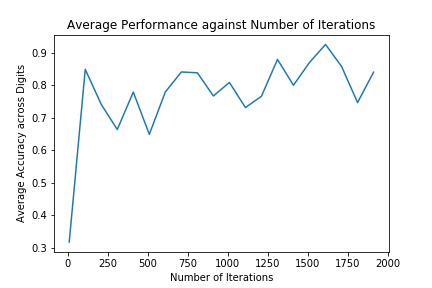
\includegraphics[]{q6/img/iterations_v1.png}
		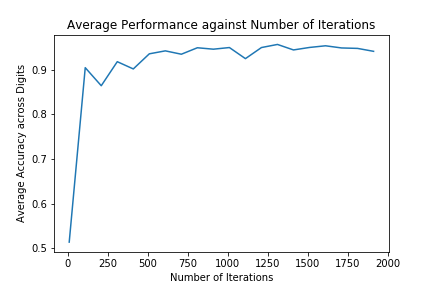
\includegraphics[]{q6/img/iterations_v2.png}
	\end{figure}

	


\subsection*{(iii)}

\end{document} 
